\documentclass{beamer}
\usepackage{advdate}
\usepackage{graphicx}

\title{Leakage Removal for Music Learning}
\author[LIU Qingyuan]{LIU Qingyuan\\Supervisors: Alia Morsi and Marius Miron}
\institute{ASPLAB 1 and 2, Music Technology Group, Universitat Pompeu Fabra}
\date{\AdvanceDate \today}

\begin{document}
\frame{\titlepage}

\begin{frame}
\frametitle{Research Movitation \& Goal}
\begin{figure}[t]
\centering
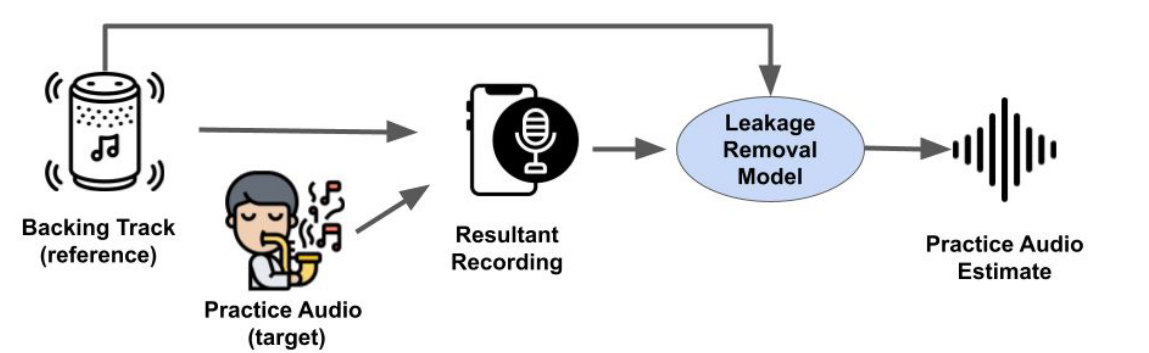
\includegraphics[width=\linewidth]{demo.png}
\end{figure}
\begin{itemize}
\item When practicing instrument, learners typically practice along with known backing tracks.
\item The recorded audio is a mixture of learners' performance and the background tracks.
\item We are trying to develop an algorithm than can remove the leakage of background tracks.
\end{itemize}
\end{frame}

\begin{frame}
\frametitle{Methodology and Work Plan}
\begin{itemize}
\item Methodology:
\begin{itemize}
\item Try to ``port'' those state-of-the-art machine learning models used in similar tasks (such as source seperation and denoising) to this task.
\end{itemize}

\item Work Plan:
\begin{itemize}
\item Gather datasets for constructing data
\item Investigate state-of-the-art machine learning models used in source separation and denoising to select the most suitable representation for the task
\item Modify nueral network architectures, then train and test
\item Study different evaluation metrics and design subjective tests (human listening test). Evaluate the newly trained model in real world data
\end{itemize}
\end{itemize}
\end{frame}
\end{document}